\documentclass{article}

\usepackage{fullpage}
\usepackage{parskip}
\usepackage{color}
\usepackage{listings}
\usepackage{amsmath}
\usepackage{graphicx}
\usepackage{caption}
\usepackage{subcaption}

\lstset{basicstyle=\ttfamily}
\lstset{keywordstyle=\ttfamily\bfseries}
\lstset{language=LISP}
\lstset{columns=fullflexible}

\begin{document}
\title{Program Synthesis for DNA Strand Displacement}
\author{Kendall Stewart, Anthony Ha, Martin Kellogg}

\maketitle

\section{Introduction}

DNA computing seeks to leverage the chemical properties
of DNA molecules as a computational substrate.
From a medical perspective, DNA computing can enable the
construction of complex devices at a cellular scale for more precise
diagnostic tests or drug delivery. From a computer architecture perspective,
DNA is capable of performing massively parallel computations with very low
power consumption.

The feasibility of DNA computing was first demonstrated by encoding the
Hamiltonian Path Problem into DNA~\cite{adelman}. This encoding was constructed
by hand, but recent work has advanced DNA strand displacement reactions as a
primitive for DNA computation, because they can implement a wide
range of algorithms and devices, including boolean circuits~\cite{strands},
oscillators~\cite{dsd}, and neural networks~\cite{strandnn}.

Because of their boolean completeness, strand displacement reactions are
theoretically capable of implementing binary arithmetic operations. However,
some operations (such as multiplication) require a large number of
boolean gates, and strand-based boolean gates do not scale as well as
silicon-based gates; even moderately-sized systems begin to suffer noise
from unwanted interactions.

Because strand displacement reactions are capable of more than just boolean
logic, an arithmetic operation can be implemented with a set of
fewer, more complex strand displacement gates. However, reasoning about the
behavior of more complex reactions is difficult for humans. We hypothesize that
a program synthesis tool equipped with appropriate semantics for strand
displacement reactions could ``discover" gates that would be difficult for a
human to find.

A formal semantics for strand displacement reactions is provided in the
description of DSD~\cite{dsd}, a programming language for specifying and
simulating DNA strand displacement circuits. Given a set of initial strand
species (reactants), DSD applies reduction rules to infer the intermediate and
final strand species (products), and creates a directed reaction graph with
edges between reactants and products, weighted by the rate of each reaction.
This graph, along with ordinary differential equations derived from the rates,
are used to simulate the strand displacement system.

Ignoring rates, the structure of the unweighted reaction graph encodes
conditions that are necessary (but not sufficient) for some product to have a
particular meaning. For instance, if all paths leading to a product include both
initial species $A$ and initial species $B$, the product could
represent $A \land B$.

As a first pass at applying program synthesis to DNA strand
displacement, we have implemented an interpreter for the semantics of
DSD in Rosette~\cite{rosette}. Our tool enables us to construct
predicates that can reason about
the structure of the resulting graph (without reaction rates). Our goal
for the quarter was to determine whether
the solver can satisfy queries such as ``given
reactant $A$ and reactant $B$, find a system of gates where the
product represents $A \land B$" (where this meaning is derived from
the graph structure, as described above).

\textcolor{red}{TODO: Paragraph summarizing results + new OR gate.}

The primary contributions of our work are:
\begin{enumerate}
\item
  An implementation in Rosette of both the detailed
  and default semantics for DSD, as an interpreter for
  strand displacement reactions.

\item
  An evaluation of this interpreter's usefulness for synthesizing
  implementations of simple boolean circuits as strand displacement
  reactions.

\item
  \textcolor{red}{A cool new gate or the like if we end up finding one.}
\end{enumerate}

\section{Overview of Our Approach}

\textcolor{red}{Describe how we took the semantics presented in the DSD paper and translated them into Rosette. A few paragraphs at most.}

DSD~\cite{dsd} is a language for specifying strand displacement
reactions.  DSD includes four semantics, which each define an
interpretation of the syntax they use to represent strand displacement
reactions, ranging from very faithful to the \emph{wetware}---the actual
DNA reactions--to very abstract. We focused on two semantics:
detailed and default. The \emph{detailed} semantics is the most faithful
to the wetware while still ignoring reaction rates, which we chose not
to model since they are defined by real-valued ordinary differential
equations, which we expected would be too expensive for the solver to
reason about. The \emph{default} semantics (named because the DSD tool
uses them by default), by contrast, combines many of the reactions
specified in the detailed semantics into abstract reactions that
are easier to reason about but less faithful to what actually happens
in practice.

The detailed semantics consists of simpler reactions than the default
semantics, but the default semantics has fewer reactions. Because we
intended to only implement the reactions we would need to demonstrate
the viability of the approach on a simple example (initially an
AND gate), we began by implementing only the reactions from the
detailed semantics that are needed to reproduce the AND gate given as
an example by DSD. We discovered, however, that because we needed many
rules (\textcolor{red}{HOW MANY?}) the performance of the solver was
unacceptable with the detailed semantics. We therefore implemented the
default semantics, instead. Our results are based on the default semantics.

\section{Algorithms and Encodings}

\subsection{Syntactic Encoding}

The core syntactic unit of the DSD language is a \emph{domain}, which is an
identifier that represents a unique sequence of DNA bases.  Identifiers ending
in a \lstinline{^} symbol represent short (also called \emph{toehold}) domains,
while all other identifiers represent long domains. The identity of the
individual bases in the sequence is left abstract, but distinct identifiers are
assumed to map to non-interfering sequences. 

DSD also specifies a \emph{complement} operation on domains, which is denoted
with a \lstinline{*} symbol after the identifier. This represents the
Watson-Crick complement of the sequence, where \lstinline{A} and \lstinline{T}
are complementary, and \lstinline{C} and \lstinline{G} are complementary.  
For example, if \lstinline{1^} represents \lstinline{ACTG}, then \lstinline{1^*}
represents \lstinline{TGAC}.

DNA molecules in solution exist in both single and double-stranded forms.
In double-stranded DNA, a sequence of bases is bound with its complementary
sequence. These forms are expressed in DSD as \emph{strands} and \emph{gates}.
A \emph{strand} is a single-stranded sequence of zero or more domains, for
example \verb;<1 2 3>;. This can also be written as the rotationally symmetric
form \verb;{3 2 1};.
A \emph{gate} is a double-stranded sequence of one or more domains,
along with single-stranded overhangs on the top and bottom of each side,
for example \verb;<1>{2}[3 4]{5}<6>;.
Two gates may also share an upper or lower strand. If \verb;G1; and \verb;G2;
are gates, the upper is written \verb;G1::G2; and the lower \verb;G1:G2;.

Our encoding of DSD's syntactic constructs is straightforward.
Long domains are represented as non-negative integers, while
short domains are non-negative integers wrapped in a \verb;toehold; struct.
The complement operation is also a \verb;struct;.
Sequences of domains are represented as lists, and strands are lists
tagged with the type (upper, lower, or double-stranded). Gates
are a five-tuple consisting of their constituent strands.
Examples syntactic encodings are shown in Table~\ref{table:encoding-example}.

\begin{table}
\begin{tabular}{|l|l|l|} \hline
Construct     & DSD Syntax    & Encoding                      \\ \hline
Long Domain   & \verb;0;      & \verb;0;                      \\ \hline
Toehold       & \verb;1^;     & \verb;(toehold 1);            \\ \hline
Complement    & \verb;1^*;    & \verb;(complement (toehold 1)); \\ \hline
Upper Strand  & \verb;<0 1^>; & \verb;(upper-strand (list 0 (toehold 1))); \\
\hline
Gate          & \verb;<1>{2^*}[3 4]{5}; &
\begin{lstlisting}
(gate
  (upper-strand (list 1))
  (lower-strand (list (complement (toehold 2))))
  (duplex-strand (list 3 4))
  (lower-strand (list 5))
  (upper-strand '()))
\end{lstlisting}
\\
\hline
\end{tabular}
\caption{Example of syntactic encoding.}
\label{table:encoding-example}
\end{table}

\subsection{Semantic Encoding}
DSD models the behavior of DNA strand displacement reactions with
\emph{reduction rules}. Each rule is a pattern-based rewrite rule
that models the conditions for and outcomes of a known reaction
involving DNA molecules. Reduction rules are also associated with
reaction rates, which model the kinetics of that chemical reaction.

To generate the reaction network for a given set of input species,
%todo put the word species before somewhere because it's pretty useful
reduction rules are applied to exhaustion (until no new species are produced).
The DSD specification refers to the set of reduction rules applied
as the level of \emph{semantic abstraction}, and they define four such levels.
The more more refined levels
use more rules, and produce more intermediate species. The 
coarser abstractions use fewer rules (and merge some rules together), thus
eliding intermediate species.

Our encoding implements the coarsest level of semantic abstraction, which DSD
refers to as the \emph{infinite} abstraction. This abstraction only has one
rule, rule RP, which describes binding interactions between two strands that can
potentially lead to a strand displacement (where a single strand is released
from a gate). The infinite abstraction also specifies that the strand
displacement itself (which is another reduction rule, RD), is merged
into the reaction.

Rules RP and RD, and an outline of their merged encoding in Rosette are shown in
Figure~\ref{figure:example-rule}. The outermost \verb;match*; expression
performs a purely syntactic match to determine whether the species are
of the correct type, and to bind their fields to variable names.

\begin{figure}

\begin{subfigure}[c]{0.5\textwidth}
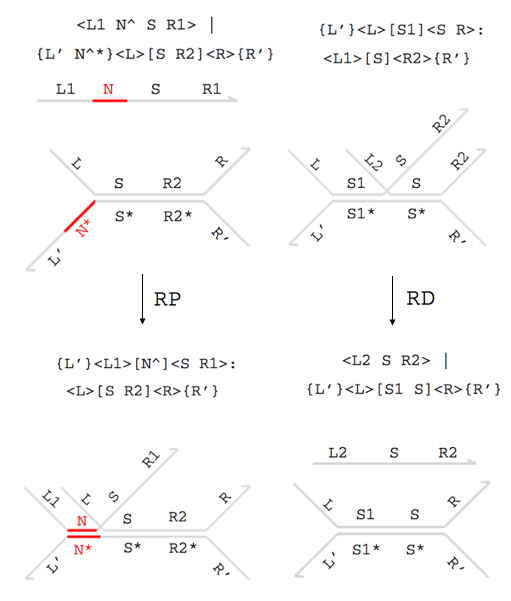
\includegraphics[width=\textwidth]{figures/rule-merge.png}
\end{subfigure}
~
\begin{subfigure}[c]{0.5\textwidth}
\begin{lstlisting}[basicstyle=\footnotesize\ttfamily]
(define (rule-rp strand-in gate-in)
  (match* (strand-in gate-in)
    [ ((upper-strand upper)

       (gate
        (upper-strand left-upper)
        (lower-strand left-lower)
        (duplex-strand duplex)
        (lower-strand right-lower)
        (upper-strand right-upper)))

      (match (toehold-search upper left-lower)
        ; no matching toehold, no reaction
        [ '() (reaction strand-in gate-in '() '()) ]

        ; matching toeholds
        [ (list ...)

          ; conditional merge with other rules
          (cond
            ...
            ; strand displacement
            [ ...
               (reaction
                strand-in gate-in
                (upper-strand ...)
                (gate ...)) ]) ]) ]

    [ (_ _) (reaction strand-in gate-in '() '()) ]))
\end{lstlisting}
\end{subfigure}
\caption{
Rules RP and RD, and their encoding as a merged rule, \lstinline{rule-rp} in
Rosette.  On the left, all identifiers (\lstinline{S}, \lstinline{R2}, etc.)
represent domain concatenations (lists of domains), except for \lstinline{N},
which represents a single toehold domain.
}
\label{figure:example-rule}
\end{figure}

The inner \verb;match; and \verb;cond;
expressions discover whether the domains of the input species satisfy
the requirements of the rule. If so, the result is a \verb;reaction;,
which is a 4-tuple containing the input strand and gate, and the
output strand and gate. The empty list is used in
cases where a product is not produced.

To produce the reaction graph, instead of applying the rule until
no new species are introduced, \textcolor{red}{Kendall fell asleep.}

\subsection{Solver-Aided Queries}

Something something \verb;choose*; something something \textcolor{red}
{Kendall fell asleep.}

\begin{figure}
\[\mathrm{isAndSystem}(g, i_1, i_2) =
\exists x \in \mathrm{strands}(g)\ .\ 
\forall p \in \mathrm{parents}(x, g)\ .\ 
\mathrm{requires}(p, i_1) \land \mathrm{requires}(p, i_2)\]
\begin{align*}
\mathrm{isOrSystem}(g, i_1, i_2) = & \ 
\exists x \in \mathrm{strands}(g)\ .
\\
& \ (\exists p \in \mathrm{parents}(x)\ .\ 
\mathrm{requires}(p, i_1) \land \lnot \mathrm{requires}(p, i_2))
\\
\land & \ 
(\exists p \in \mathrm{parents}(x)\ .\ 
\lnot \mathrm{requires}(p, i_1) \land \mathrm{requires}(p, i_2))
\end{align*}
\caption{
First-order predicates over a reaction network
$g$ given input strands $i_1$ and $i_2$.
}
\end{figure}

\textcolor{red}{
Needs some more flow/context, could be in this subsection,
or in section 2 with less detail
\\
As we were working on writing the rule functions, we originally were
verifying the rules through traditional \emph{ad hoc} testing. But,
since we were working in Rosette, once synthax was defined for domain
concatenations we were able to write a series of tests that verify
properties of rules (such as that the presence of the products in the
result implies the presence of the reactants in the original system)
for bounded domain concatenations of up to some size $k$ (because our
tests were being run on a CI server on each commit, they were
typically restricted to $k=2$ or $k=3$). We found the ability to write
these tests to be a very useful property of a solver-aided language;
we were much more confident that the (complex) rule implementations
were correct once we had verified them for small domain
concatenations.
}


\section{Results}

\textcolor{red}{Description of AND and OR gate synthesis, limitations, etc}

\section{Teamwork}

To ensure that all three of us were involved in developing the encoding of
strand displacement reactions we used, much of the core infrastuctural code
that defines the encoding was developed by all three of us working on a single
screen. Once we had defined the core encoding, each team member worked on
making use of it in a particular way: Kendall, as the domain expert, worked
on implementing the rules and refining the encoding to perform better; Anthony
worked on building a implementing a normalization procedure (which required
some modifications to the encoding, as well) and a pretty printer/parser;
Martin created a test infrastructure (including a continuous integration server)
and then on writing verification procedures for the rules Kendall was
implementing (i.e. solver-aided exhaustive tests).

\section{Course Topics}

This project made heavy use of a solver-aided language: it is entirely dependent
on Rosette. In particular, we needed Rosette's ability to angelically execute
our symbolic programs (which represent reactions) and produce reactants that
cause the programs (reactions) to have the desired behavior---our synthesis
task. We also used bounded verification to test that our more complex
rules were correct. All topics we required were covered by the class.

\begin{thebibliography}{9}

\bibitem{adelman}
L. M. Adleman,
“Molecular computation of solutions to combinatorial problems,”
Science, vol. 266, no. 5187, pp. 1021–1024, Nov. 1994.

\bibitem{strands}
D. Y. Zhang and G. Seelig,
“Dynamic DNA nanotechnology using strand-displacement reactions,”
Nature Chemistry, vol. 3, no. 2, pp. 103–113, Feb. 2011.

\bibitem{dsd}
M. R. Lakin, S. Youssef, L. Cardelli, and A. Phillips,
“Abstractions for DNA circuit design,”
Journal of The Royal Society Interface, vol. 9, no. 68, Jul. 2011.

\bibitem{strandnn}
L. Qian, E. Winfree, and J. Bruck, “Neural network computation with DNA strand
displacement cascades,” Nature, vol. 475, no. 7356, pp. 368–372, Jul. 2011.

\bibitem{rosette}
  E. Torlak and R. Bodik, “A lightweight symbolic virtual machine for solver-aided host languages,” Programming Language Design and Implementation (PLDI), vol. 49, no. 6, pp. 530-541, 2014.

\end{thebibliography}

\end{document}
